\chapter{DevOps\label{devops}}

DevOps:illa tarkoitetaan ohjelmistokehityksen ja IT-toimintojen yhdistämistä.
DevOps:iin liitetään usein jatkuva integraatio ja toimitus sekä automaatio ja laadunvalvonta \cite{Jabbari16, Leite19}.
DevOps:ia käsitteenä voidaan tarkastella ajattelutapana tai käytännön ohjelmistotuotannon toimintamallina.

DevOps ajattelutapana pyrkii ohjelmistokehityksen ja IT-toimintojen jaon välttämiseen ja yhteistoiminnan mahdollistavan kulttuurin rakentamiseen \cite{Klein21}.
DevOps toimintamallina taas keskittyy käytännön toimiin ja teknologioihin, jotka mahdollistavat DevOps-ajattelutavan mukaisen ohjelmistotuotannon.
Tässä tutkielmassa keskitytään aiheen käsittelyyn käytännön toimintamallin kautta.

\section{DevOps-toimintamalli}

DevOps-toimintamalli painottaa jatkuvaa integraatiota ja toimitusta sekä laadunvalvontaa käyttäen standardisoituja automaattisia menetelmiä \cite{Leite19}.
Kuva~\ref{fig:devops} visualisoi DevOps-toimintamallin eri vaiheita.
Kehitys- ja operaatiovaiheet tapahtuvat limittäin ja koko prosessi voidaan suorittaa useita kertoja päivässä automatisoidun julkaisuputken avulla.

\begin{figure}[ht]
\begin{center}
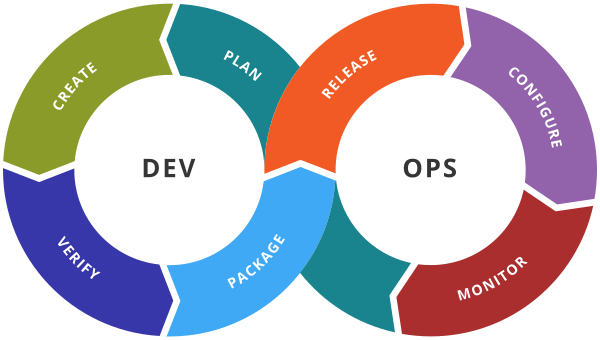
\includegraphics[width=0.6\textwidth]{figures/devops_toolchain.png}
\caption{DevOps-toimintamallin vaiheet.\cite{Wikimedia23}\label{fig:devops}}
\end{center}
\end{figure}

DevOps-toimintamallin vaiheet ja niistä käytetyt termit vaihtelevat lähteestä riippuen, mutta tämän tutkielman osalta käytetään seuraavia vaiheita \cite{Alnafessah21}:

\begin{itemize}
\item Määrittely (engl. \textit{plan}): Ohjelmistotuotannon tavoitteiden määrittely sekä päivitysten ja julkaisuiden alustava suunnittelu.
\item Kehitys (engl. \textit{create, develop}): Määrittelyn mukainen ohjelmisto- ja infrastruktuurikoodin kehitys nopealla versiohallintaan viennillä.
\item Varmennus (engl. \textit{verify, test}): Jatkuva koodin automaattinen testaus ja koodin manuaalinen arviointi tarvittaessa.
\item Julkaisu (engl. \textit{release, deploy}): Uuden ohjelmakoodin julkaisu tuotantoympäristöön ja tuotantoalustan konfiguraatio.
\item Operointi (engl. \textit{operate, configure}): Julkaisun jälkeinen palvelun hallinnointi, resurssien hallinta ja palvelun skaalautuminen.
\item Monitorointi (engl. \textit{monitor}): Palvelun suorituskyvyn ja lokien seuranta, ongelmatilanteisiin reagointi.
\end{itemize}

\section{Jatkuva integraatio ja toimitus}

Jatkuva integraatio ja toimitus (engl. \textit{continuous integration and continuous deployment, CI/CD}) on keskeinen osa DevOps-toimintamallia \cite{Jabbari16, Leite19}. Jatkossa tutkielmassa käsitteisiin viitataan vakiintuneilla lyhenteillä CI ja CD.

CI viittaa koodimuutosten vientiin versionhallintaan nopealla tahdilla ja muutosten automaattiseen testaukseen sen yhteydessä.
CD taas tarkoittaa CI:n seurauksena validoidun koodin automaattista julkaisua tuotantoympäristöön tai sitä muistuttavaan testiympäristöön \cite{Shahin17}.
CI/CD mahdollistaa näin tehokkaan laadunvalvonnan ja ohjelmiston nopean julkaisusyklin.

\begin{figure}[ht]
\begin{center}
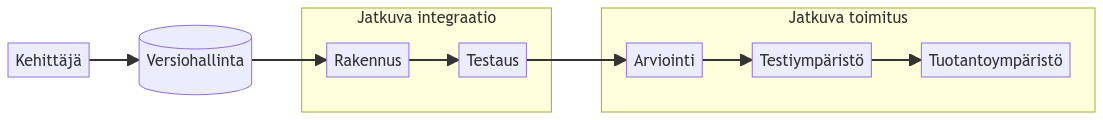
\includegraphics[width=0.8\textwidth]{figures/cicd-pipeline.png}
\caption{Jatkuvan integraation ja toimituksen vaiheet.\label{fig:cicd}}
\end{center}
\end{figure}

Kuva \ref{fig:cicd} esittää esimerkin mahdollisesta CI/CD-putkesta. CI/CD käynnistyy kehittäjän puskiessa uuden koodimuutoksen versiohallintaan.
CI:n aikana uusi version sovelluksesta rakennetaan päivitetystä koodista ja uudelle versiolle suoritetaan automaattiset testit.
Automaattiset testit läpäissyt koodi voidaan tarvittaessa katselmoida ja sovelluksen uusi versio julkaistaan vaiheittain testi- ja tuotantoympäristöihin osana CD:tä.

\section{Haasteet}

DevOps-toimintamalliin perustuva ohjelmistotuotanto luo uusia haasteita.
CI/CD ja toimintamallin vaiheiden seuraaminen nopealla syklillä vaatii automaatiota ja vaiheiden helppoa toistettavuutta \cite{Jabbari16, Leite19}.
Ohjelmistokehittäjien perehdyttäminen DevOps:in mukaisiin toimintatapoihin ja teknologiohiin on yksi haasteista.
Myös DevOps-toimintamallin käyttöönotto sekä toimintamallin seurannan laadun arvioiminen on haastavaa \cite{Leite19}.
Haasteissa painottuvat erityisesti inhimilliset tekijät kuten kommunikaatiohaasteet ja muutosvastarinta \cite{Kalliosaari16}.
Teknisen puolen haasteita ovat taas ohjelmistoinfrastruktuurin hallinta, kuten monimutkaiset kehitys- ja tuotantoympäristöt \cite{Khan22, Kalliosaari16}.

DevOps-toimintamallin käyttöönoton yhteydessä on arvioitava erilaisten teknologioiden soveltuvuuttaa osaksi mallin mukaista ohjelmistotuotantoa.
Sopivilla teknologiavalinnoilla voidaan vähentää ohjelmistoinfrastruktuurin monimutkaisuutta.
Yksi näistä teknologiavalinnoista on julkaisutavan valinta.
Automaation ja toistettavuuden kannalta ratkaisuksi sopisi esimerkiksi virtuaalikoneet tai konttiteknologia \cite{Dua14}.
Konttiteknologiaa ja konttien orkestrointia voidaan käyttää onnistuneesti osana DevOps-toimintamallia \cite{Kang16, Narasimhulu23}.
Seuraavaksi käsitellään näitä aiheita ja arvioidaan niiden yhteensopivuuttaa DevOps-toimintamallin kanssa.

% Expand into more challenges and especially benefits e.g. Why should the reader or anyone use DevOps
